\documentclass[a4paper, 12pt, english]{article}

\usepackage[utf8]{inputenc}
\usepackage{amsmath,amssymb}
\usepackage{graphicx}
\usepackage{subfig}
\usepackage[colorinlistoftodos]{todonotes}

\usepackage{indentfirst}
\usepackage{verbatim}
\usepackage{textcomp}
\usepackage{gensymb}

\usepackage{relsize}

\usepackage{lipsum}% http://ctan.org/pkg/lipsum
\usepackage{xcolor}% http://ctan.org/pkg/xcolor
\usepackage{xparse}% http://ctan.org/pkg/xparse
\NewDocumentCommand{\myrule}{O{1pt} O{2pt} O{black}}{%
  \par\nobreak % don't break a page here
  \kern\the\prevdepth % don't take into account the depth of the preceding line
  \kern#2 % space before the rule
  {\color{#3}\hrule height #1 width\hsize} % the rule
  \kern#2 % space after the rule
  \nointerlineskip % no additional space after the rule
}
\usepackage[section]{placeins}

\usepackage{booktabs}
\usepackage{colortbl}%
   \newcommand{\myrowcolour}{\rowcolor[gray]{0.925}}
   
\usepackage[obeyspaces]{url}
\usepackage{etoolbox}
\usepackage[colorlinks,citecolor=black,urlcolor=blue,bookmarks=false,hypertexnames=true]{hyperref} 

\usepackage{geometry}
\geometry{
	paper=a4paper, % Change to letterpaper for US letter
	inner=0.5cm, % Inner margin
	outer=1cm, % Outer margin
	bindingoffset=.5cm, % Binding offset
	top=2cm, % Top margin
	bottom=2cm, % Bottom margin
	%showframe, % Uncomment to show how the type block is set on the page
}

\usepackage{float}

\usepackage{amsmath,amsfonts,pxfonts}

\usepackage{listings}
\lstset{
  escapeinside={(*}{*)},
}
% MATLAB code formatting
\lstdefinestyle{matlab}{
    language=Matlab,
    basicstyle=\scriptsize\ttfamily,
    keywordstyle=\color{blue},
    commentstyle=\color{green!40!black},
    stringstyle=\color{red},
    showstringspaces=false,
    numbers=left,
    numberstyle=\tiny,
    numbersep=5pt,
    tabsize=2,
    breaklines=true,
    breakatwhitespace=true
}
% MATLAB command window formatting
\lstdefinestyle{commandstyle}{
    basicstyle=\scriptsize\ttfamily,
    numbers=none,
    showstringspaces=false,
    breaklines=true,
    frame=single,
    frameround=fttt,
    backgroundcolor=\color{gray!10},
    xleftmargin=0.5cm,
    xrightmargin=0.5cm
}


\usepackage{multicol,caption}
\newenvironment{Figure}
  {\par\medskip\noindent\minipage{\linewidth}}
  {\endminipage\par\medskip}
\usepackage{array}

\newcommand{\highlight}[1]{\textcolor{blue}{\texttt{#1}}}

\usepackage[backend=biber, style=ieee]{biblatex}
\addbibresource{references.bib}

\graphicspath{{images/}}

\setlength {\marginparwidth }{2cm} 

\newcommand{\usection}[1]{\section*{#1}
\addcontentsline{toc}{section}{\protect\numberline{}#1}}

\newcommand{\usubsection}[1]{\subsection*{#1}
\addcontentsline{toc}{subsection}{\protect\numberline{}#1}}

\newcommand{\usubsubsection}[1]{\subsubsection*{#1}
\addcontentsline{toc}{subsubsection}{\protect\numberline{}#1}}

\usepackage{bm}
%*******************************************************************************%
%************************************START**************************************%
%*******************************************************************************%
\begin{document}

%************************************TITLE PAGE**************************************%
\begin{titlepage}
\begin{center}
\textbf{\LARGE Alexandria University}\\[0.5cm] 
\textbf{\large FACULTY OF ENGINEERING}\\[0.2cm]
\vspace{20pt}

\includegraphics{logo.png}\\[1cm]
\par
\vspace{20pt}
\textbf{\Large EEC-461 Antenna Engineering}\\
\vspace{15pt}
\myrule[1pt][7pt]
\textbf{\LARGE Linear Antenna}\\
%\vspace{15pt}
%\textbf{\large Analysis of 3G and 4G}\\
\myrule[1pt][7pt]
\vspace{25pt}
\textbf{\large \hspace{50pt}Student Name \hspace{60pt} Student ID}\\
Ahmed Osama Mohamed Afifi \hspace{60pt} 20010038 \\

\vspace{45pt}
\textbf {\large Lecturer in charge:}\\[0.2cm]
\Large {Prof Dr. Said E. El-Khamy}\\[0.1cm]
\end{center}

\par
\vfill
\begin{center}
\textbf{Submission Date : 31/10/2024}\\
\end{center}

\end{titlepage}

%************************************TABLE OF CONTENTS**************************************%

%  %Summary
  \newpage
  \hypersetup{linkcolor=black}
  \tableofcontents
%  \thispagestyle{empty}
  %End Summary

%********************************%
%***********SECTION 1************%
%********************************%
\newpage
\section{Introduction}
Linear antennas, especially dipole antennas, are fundamental components in the world of wireless communication and radio technology. A linear antenna typically consists of two conductive elements arranged in a straight line, which allows it to efficiently transmit and receive electromagnetic waves. Among the various types of antennas, the linear dipole is one of the simplest designs, making it a common choice for both theoretical studies and practical applications. \\

The performance of a linear dipole antenna is heavily influenced by its length in relation to the wavelength of the signals it handles. As the dipole length increases, various characteristics such as gain, radiation resistance, and bandwidth change significantly. Understanding these relationships is essential for optimizing antenna designs for specific applications, including broadcasting, mobile communications, and radar systems. \\

In this report, It is required to analyze long linear dipole antennas by examining how dipole length $(l/\lambda)$ affects the gain $(G_0)$ and radiation resistance $(R_{rad})$. 

%********************************%
%***********SECTION 2************%
%********************************%
\section{Mathematical Background}
Given the electric field equation:
\begin{equation}
    \left|{E}_{\theta} \right| = \frac{{\eta}{\left| {I}_{m} \right|}}{{2}{\pi}{r}} \left[ \frac{\cos{\left(\frac{{\beta}{l}}{2} cos(\theta)\right)} - \cos{\left(\frac{{\beta}{l}}{2}\right)}}{\sin{\left(\theta\right)}} \right] {V}/{m}
\end{equation}

The power pattern can be obtained finding ${P}_{av}$, as
\[
{P}_{av} = \frac{1}{2} \Re\left[ \Vec{E} \times \Vec{H^*} \right]
 = \frac{1}{{2}{\eta}} \left| E \right| ^ 2
\]
\begin{equation}
\label{eq1}
{P}_{av} = \frac{\eta}{8 {\pi}^{2} {r}^{2}} \left| {I}_{m} \right| ^{2} \left[ \frac{\cos{\left(\frac{{\beta}{l}}{2} \cos{(\theta)}\right)} - \cos{\left(\frac{{\beta}{l}}{2}\right)}}{\sin{\left(\theta\right)}} \right] ^ {2} {W}/{{m}^{2}}    
\end{equation}


The total radiated power can be obtained finding ${W}_{T}$, as
\[
{W}_{T} = \oiint \Vec{{P}_{av}}.d\Vec{S}
= \iint {P}_{av} {r}^{2} \sin{\left(\theta\right)} d\phi d\theta
\]

\[
{W}_{T} = \frac{\eta}{8} {\pi}^{2} \left| {I}_{m} \right| ^{2} \int_{\phi=0}^{\phi=2\pi} \int_{\theta=0}^{\theta=\pi} \frac{\left[ \cos{\left(\frac{{\beta}{l}}{2} \cos{(\theta)}\right)} - \cos{\left(\frac{{\beta}{l}}{2}\right)} \right] ^ {2}}{{{r}^{2}}{\sin{\left(\theta\right)}}} d\phi d\theta
\]

\begin{equation}
    \begin{split}
        {W}_{T} &= \eta \frac{\left| {I}_{m} \right| ^ {2}}{{4}{\pi}} \left\{ {C} + \ln{\left( {\beta}{l} \right)} - {{C}_{i}}\left( {\beta}{l} \right) + \frac{1}{2} \sin{\left( {\beta}{l} \right)} \left[ {{S}_{i}}\left( {2}{\beta}{l} \right) - {2}{{S}_{i}}\left( {\beta}{l} \right) \right] \\&+ \frac{1}{2} \cos{\left( {\beta}{l} \right)} \left[ {C} + \ln{\left( \frac{{\beta}{l}}{2} \right)} + {{C}_{i}}\left( {2}{\beta}{l} \right) - {2}{{C}_{i}}\left( {\beta}{l} \right) \right] \right\} {W}
    \end{split}
\end{equation}

where, 
\[ {C} = \lim_{{n}\to\infty} \left( - \ln{\left( n \right)} + \sum_{k=1}^{n} \frac{1}{k} \right) \approx 0.577216  \quad \textrm{(Euler's constant)} \]
\[ {{C}_{i}}{\left( {x} \right)} = - \int_{x}^{\infty} \frac{\cos{\left( y \right)}}{y} dy = \int_{\infty}^{x} \frac{\cos{\left( y \right)}}{y} dy = \int_{0}^{x} \frac{{{1} - \cos{\left( y \right)}}}{y} dy \]
\[ {{S}_{i}}{\left( {x} \right)} = \int_{0}^{x} \frac{\sin{\left( y \right)}}{y} dy \]

The radiation resistance ${R}_{rad}$ can be obtained as:
\begin{equation}
\begin{split}
    \label{eq3}
    {R}_{rad} & = \frac{{2}{{W}_{T}}}{\left| {{I}_{m}} \right| ^ {2}} \\
    & = \frac{\eta}{{2}{\pi}} \left\{ {C} + \ln{\left( {\beta}{l} \right)} - {{C}_{i}}\left( {\beta}{l} \right) + \frac{1}{2} \sin{\left( {\beta}{l} \right)} \left[ {{S}_{i}}\left( {2}{\beta}{l} \right) - {2}{{S}_{i}}\left( {\beta}{l} \right) \right] + \frac{1}{2} \cos{\left( {\beta}{l} \right)} \left[ {C} + \ln{\left( \frac{{\beta}{l}}{2} \right)} + {{C}_{i}}\left( {2}{\beta}{l} \right) - {2}{{C}_{i}}\left( {\beta}{l} \right) \right] \right\}
\end{split}
\end{equation}

The gain ${G}_{0}$ can be obtained as:
\begin{equation}
    \begin{split}
        {G}_{0} & = \frac{{P}_{max}}{{W}_{T}} {{4}{\pi}{{r^{2}}}} \\
        & = {2} \frac{\left[ \frac{\cos{\left(\frac{{\beta}{l}}{2} \cos{(\theta)}\right)} - \cos{\left(\frac{{\beta}{l}}{2}\right)}}{\sin{\left(\theta\right)}} \right] ^ {2}}{\left\{ {C} + \ln{\left( {\beta}{l} \right)} - {{C}_{i}}\left( {\beta}{l} \right) + \frac{1}{2} \sin{\left( {\beta}{l} \right)} \left[ {{S}_{i}}\left( {2}{\beta}{l} \right) - {2}{{S}_{i}}\left( {\beta}{l} \right) \right] + \frac{1}{2} \cos{\left( {\beta}{l} \right)} \left[ {C} + \ln{\left( \frac{{\beta}{l}}{2} \right)} + {{C}_{i}}\left( {2}{\beta}{l} \right) - {2}{{C}_{i}}\left( {\beta}{l} \right) \right] \right\}} \\
        & = \frac{{2} {F(\theta)|_{max}}}{Q}
    \end{split}
\end{equation}

where, 
\begin{equation}
    \begin{split}
        {F}{(\theta, \phi)} = {F}{(\theta)} &= \left[ \frac{\cos{\left(\frac{{\beta}{l}}{2} \cos{(\theta)}\right)} - \cos{\left(\frac{{\beta}{l}}{2}\right)}}{\sin{\left(\theta\right)}} \right] ^ {2} \\
        &= \left[ \frac{\cos{\left(\pi \frac{l}{\lambda} \cos{(\theta)}\right)} - \cos{\left(\pi \frac{l}{\lambda}\right)}}{\sin{\left(\theta\right)}} \right] ^ {2}
    \end{split}
\end{equation}


\begin{equation}
    \begin{split}
        {Q} &= \left\{ {C} + \ln{\left( {\beta}{l} \right)} - {{C}_{i}}\left( {\beta}{l} \right) + \frac{1}{2} \sin{\left( {\beta}{l} \right)} \left[ {{S}_{i}}\left( {2}{\beta}{l} \right) - {2}{{S}_{i}}\left( {\beta}{l} \right) \right] + \frac{1}{2} \cos{\left( {\beta}{l} \right)} \left[ {C} + \ln{\left( \frac{{\beta}{l}}{2} \right)} + {{C}_{i}}\left( {2}{\beta}{l} \right) - {2}{{C}_{i}}\left( {\beta}{l} \right) \right] \right\} \\
        &= \left\{ {C} + \ln{\left( {2}{\pi}\frac{l}{\lambda} \right)} - {{C}_{i}}\left( {2}{\pi}\frac{l}{\lambda} \right) + \frac{1}{2} \sin{\left( {2}{\pi}\frac{l}{\lambda} \right)} \left[ {{S}_{i}}\left( {4}{\pi}\frac{l}{\lambda} \right) - {2}{{S}_{i}}\left( {2}{\pi}\frac{l}{\lambda} \right) \right] \\&+ \frac{1}{2} \cos{\left( {2}{\pi}\frac{l}{\lambda} \right)} \left[ {C} + \ln{\left( {\pi}\frac{l}{\lambda} \right)} + {{C}_{i}}\left( {4}{\pi}\frac{l}{\lambda} \right) - {2}{{C}_{i}}\left( {\beta}{l} \right) \right] \right\}
    \end{split}
\end{equation}

\newpage
%********************************%
%***********SECTION 3************%
%********************************%
\section{Matlab Code}
\begin{lstlisting}[style=matlab,caption={Matlab code},captionpos=b]
% |E_(*$\theta$*)| = ((*$\eta$*) * I_m) / (2 (*$\pi$*) r) { [cos(((*$\beta$*)l/2)cos((*$\theta$*))) - cos((*$\beta$*)l/2)] / sin((*$\theta$*)) }
% P_max = (|E_(*$\theta$*)| ^ 2) / (2 * (*$\eta$*))
% W_T = (*$\iint$*) P . dS
%     = ((*$\eta$*) * I_m ^ 2) * Q / (4 (*$\pi$*)) 
% G_0 = (4 (*$\pi$*) r ^ 2) P_max / W_T
%     = 2 F((*$\theta$*))|_max / Q
% R_rad = 2 W_T / (I_m ^ 2)
%       = { (*$\eta$*) / (2 (*$\pi$*)) } Q

dipole = linspace(0, 10, 1000);
theta = linspace(0, pi, 1000);
F_max = zeros(1, length(dipole));
for i = 1:length(dipole)
    F_max(i) = max(((cos(pi .* dipole(i) .* cos(theta)) - cos(pi .* dipole(i))) ./ (sin(theta))) .^ 2);
end
C = double(eulergamma);
Q = C + log(2 .* pi .* dipole) - cosint(2 .* pi .* dipole) ...
    + 0.5 .* sin(2 .* pi .* dipole) .* (sinint(4 .* pi .* dipole) - 2 .* sinint(2 .* pi .* dipole)) ...
    + 0.5 .* cos(2 .* pi .* dipole) .* (C + log(pi .* dipole) + cosint(4 .* pi .* dipole) - 2 .* cosint(2 .* pi .* dipole));

G = 2 .* F_max ./ Q;
R_rad = 60 .* Q;
xlabel('Dipole length \itl \rm(wavelengths)');
yyaxis right
plot(dipole, G, 'LineWidth', 3);
ylabel('\itG_{0} \rm(dimensionless)');
yyaxis left
plot(dipole, R_rad, '--', 'LineWidth', 3);
ylabel('\it{R_rad} \rm(ohms)');
legend('R_rad (ohms)','G_0 (dimensionless)')
\end{lstlisting}
%********************************%
%***********SECTION 4************%
%********************************%
\section{Results}
\begin{figure}[H]
    \centering
    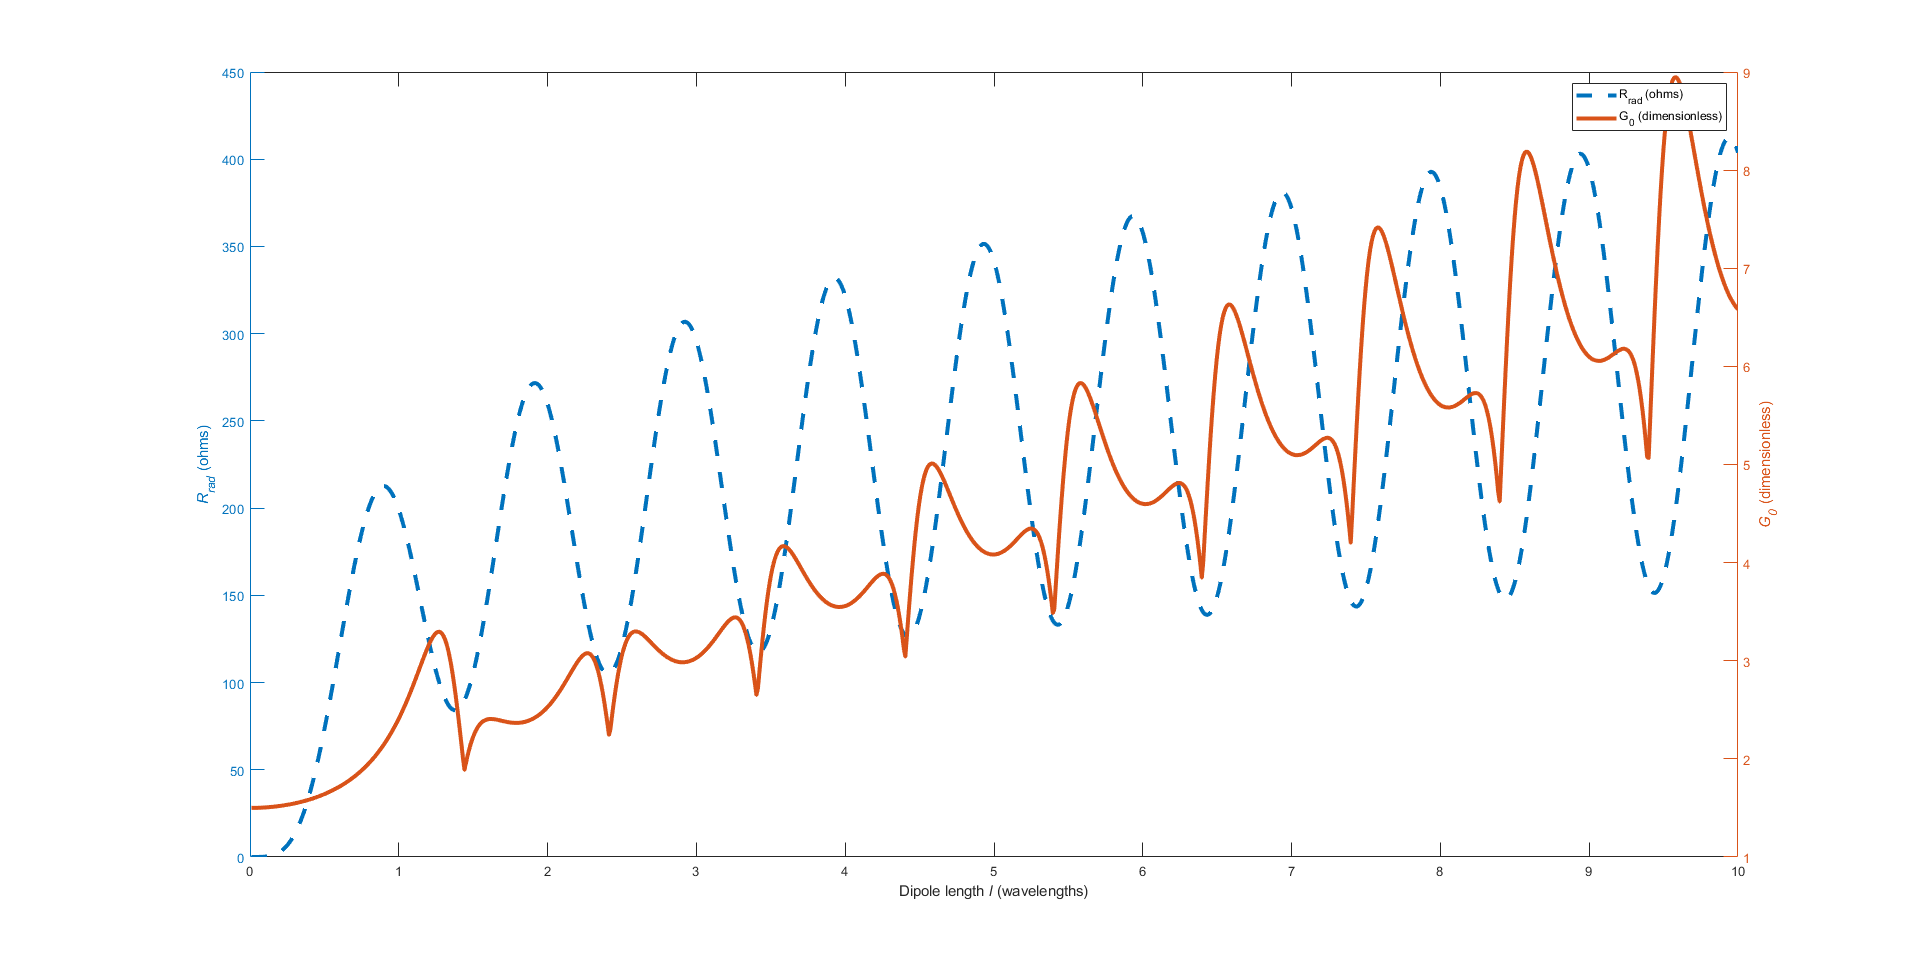
\includegraphics[width=\linewidth]{images/linearAntenna.png}
    \caption{Radiation resistance and gain of a thin dipole with sinusoidal current distribution}
\end{figure}

\end{document}